\section{The sample}
\label{sec:sample}

This search covers \NWindows{} spectral windows toward \NStars{} stars in
\NSystems{} systems within 40\,pc, drawn from \NEB{} public ALMA execution
blocks and \TotalDataTB\,TB of raw data put through one pipeline:
\StTelHours\,h of telescope time, and \LdgCensusHours\,h summed over
windows. That set is the \emph{primary census}, over which every sensitivity,
every expectation and every limit here is computed. It holds \MtCrossACen{} of
the \EvNCrossRaw{} threshold crossings this paper reports; \LdgNCrossB{} more
are coarse-channel crossings of the same census lying in the one execution
block that fails the data-quality criterion of \S\ref{sec:summary}, reported
apart for that reason and not because they fall outside it; and the remaining
\CeNTailCross{} lie in an \emph{archival tail} of blocks searched after the
census was closed, toward stars it already holds, which are not tabulated
window by window and enter no expectation. Three further sets enter no census
statistic and are reported where their results are
(\S\ref{sec:holdoutsearch}): an \emph{archival extension}, a larger harvest of
blocks toward the same stars; a reserved \emph{hold-out}, set aside by the
identifier rule of Appendix~\ref{sec:heldout}; and a control beyond
40\,pc. Table~\ref{tab:blockledger} names every set in rows that sum, and
Table~\ref{tab:counts} resolves every count of windows, crossings and systems
into the set it is counted over.

\emph{Star} means one stellar component, \emph{system} a bound group
counted once however many of its components were observed, and \emph{target}
one ALMA pointing.

The census is two experiments, divided on native channel width, which is what
the search statistic and the completeness calibration both depend on.
\emph{Class~A} is the \NWinA{} fine-channel windows toward \LdgClassAStars{}
stars in \NSysClassA{} systems, of which \EtaDriftAOk{} are channelised finely
enough for the searched drift to cross a channel and \EtaDriftALo{} are not
(\S\ref{sec:statistic}); every sensitivity and exclusion quoted here refers to
Class~A unless stated otherwise. \emph{Class~B} is the remaining \NWinB{}
coarse-channel windows, which support a secondary search for an unresolved
spectral excess. The division is unambiguous because the channelisation of the
sample is bimodal: the widest fine channel is \ScChanFineMaxMHz\,MHz and the
narrowest coarse one \ScChanCoarseMinMHz\,MHz, a factor of \ScChanGapFac{} with
nothing between them.

Every inclusion criterion was applied by query. A star enters if its Gaia~DR3
parallax is at least 25\,mas, measured to better than \PlxAdqlPct{} per cent --
a clause that never binds, the worst fractional parallax error among the stars
searched being \SfPlxWorstPct{} per cent -- and if its proper-motion-corrected
position at the observation epoch falls inside the quoted field of view of at
least one public execution block. Distances are direct inversions,
$d=1/\varpi$, and the star need not sit at the pointing centre. One further
rule applies to the window and not to the star: a window is kept only where the
primary-beam response at the star is at least \BmFloorResp, the offset at which
the Gaussian adopted here and the response of a blocked circular aperture part
by \BmFloorTolPct{} per cent on the compact-array dish, the binding one of the
two. It removes nothing, in the census or in the archival coverage beyond it,
but it does not stand clear of the distribution: the furthest window from a
pointing centre lies at \ExCWorstExt\,$\lambda/D$ against a limit at
\BmFloorC\,$\lambda/D$, and the windows it is nearest are the off-axis ones on
$\epsilon$~Eridani, which the survey searches. The quoted field of view is
optimistic: of the \NCensus{} work-list entries the query returns, only
\NGenuinelyCovered{} stars prove to be contained by a public field, and
\NStars{} of those yielded a searchable window. One target has no catalogue
name -- a serendipitous field star that appears throughout as \BkAlmaName,
Gaia~DR3 \BkAlmaGaia, an \BkAlmaSpType{} dwarf at \BkAlmaDistPc\,pc with no
measured systemic velocity.

Disc, planet and colour enter as descriptive metadata only. One exclusion,
though, is a property of the catalogue and not of the sky: a Gaia~DR3 parallax
needs a Gaia~DR3 source and the brightest stars have none -- every one of the
\BsNBright{} stars in this volume brighter than \BsBrightMag{} magnitude is
absent from DR3 astrometry -- so \BsNGap{} of the
\BsNVol{} Hipparcos stars in this volume whose own parallaxes meet the criteria
above never reached the work list -- \BsGapNBright{} of them brighter than
Hp~\BsGapMagCut{} and \BsGapNFaint{} fainter, a loss saturation does not
explain. Of those, \BsNAlmaWord{} lie inside a public field of view --
\BsStarList{} -- and hold \BsNWinA{} fine-channel and \BsNWinB{} coarse-channel
windows, \BsRawTB\,TB of raw data in \BsNEB{} execution blocks, none of it
searched here, Sirius~A among them since the \BsSirNEBWord{} blocks that put
Sirius~B in this census are pointed at it. A search of this volume should admit
these stars on Hipparcos astrometry where Gaia has none.


\subsection{The archival selection}
\label{sec:bias}

This sample was not designed: it is whatever previous ALMA programmes happened
to observe among the stars Gaia~DR3 catalogues, and \PctDiscProposal{} per cent
of the stars searched were targeted under a debris-disc or planet-formation
proposal. Table~\ref{tab:selfunc} measures the bias against a volume-limited
reference census of which the searched stars are a subset, both columns the
same Gaia~DR3 selection -- $\varpi>0$, $\sigma_\varpi/\varpi\le\SfPlxCutDec$
and $1/\varpi\le40$\,pc, \SfCensusN{} objects -- and both classified by one
rule, in which BP$-$RP colour sets the class and the absolute $G$ magnitude
separates the degenerates that colour alone would place among the A~stars, so
that every ratio below is like against like. It reaches \SfCensusNCol{} census
objects and \SfNClassified{} of the \SfNStar{} searched stars, the other
\SfNNoColour{} carrying no Gaia BP or RP photometry; both columns are
Gaia-defined, so neither contains the bright stars above and the ratios are
internally consistent without them.

Distance is the dominant selection effect: stars within 5\,pc are
over-represented by a factor \SfTopRatio, and the enhancement falls
monotonically with distance to a factor of two \emph{under}-representation
beyond 30\,pc. Colour comes second -- A~stars by about \SfARatio{} and F and G
stars by factors of three, because those are the stars with bright debris
discs; for the A~stars that factor is a floor, the Gaia requirement being
itself colour-selective and removing stars as blue as an A~star at
\BsEarlyRatio{} times its rate among all the others. M~dwarfs are depleted:
\SfMSearched{} of the \SfNStar{} searched stars, a factor \SfMRatio{} of their
share of the reference census, and only \SfMClassAStars{} of them carry
fine-channel coverage at all. Coverage is concentrated too, \ConcThreeWin{} of
the \NWindows{} windows coming from \ConcThreeSys{} systems. No statement in
this paper is therefore an occurrence rate for the solar neighbourhood, and the
selection acts hardest on exactly the targets a designed search would pick: of
the \CsIntNRow{} sample systems within 15\,pc with a confirmed planet,
\CsIntNoClassA{} carry no Class~A coverage and so no drift-resolving limit.

%% GENERATED by selfunc_v411.py -- do not hand-edit.
\begin{table}
\centering
\scriptsize
\setlength{\tabcolsep}{4pt}
\caption{Selection function of the 90 searched stars against the volume-limited Gaia~DR3 census of \S\ref{sec:bias}. ``Ratio'': the searched over the census column fraction.}
\label{tab:selfunc}
\begin{tabular}{@{}lrrr@{}}
\toprule
Property & Census & Searched & Ratio \\
\midrule
\multicolumn{4}{@{}l}{Distance} \\
\quad $d\le5$\,pc & 48 (0.3\%) & 13 (14.4\%) & 52.9 \\
\quad 5--10\,pc & 240 (1.4\%) & 13 (14.4\%) & 10.6 \\
\quad 10--20\,pc & 2069 (11.8\%) & 18 (20.0\%) & 1.7 \\
\quad 20--30\,pc & 5391 (30.7\%) & 19 (21.1\%) & 0.7 \\
\quad 30--40\,pc & 9818 (55.9\%) & 27 (30.0\%) & 0.5 \\
\midrule
\multicolumn{4}{@{}l}{Colour class$^{a}$} \\
\quad A & 61 (0.4\%) & 5 (6.2\%) & 17.2 \\
\quad F & 473 (2.8\%) & 8 (10.0\%) & 3.6 \\
\quad G & 978 (5.8\%) & 15 (18.8\%) & 3.2 \\
\quad K & 2221 (13.2\%) & 11 (13.8\%) & 1.0 \\
\quad M & 13\,082 (77.8\%) & 41 (51.2\%) & 0.7 \\
\midrule
\multicolumn{4}{@{}l}{Other axes} \\
\quad Confirmed planet hosts$^{b}$ & 26 (15.5\%) & 24 (26.7\%) & 1.7 \\
\quad White dwarfs$^{a}$ & 463 (2.7\%) & 8 (9.1\%) & 3.4 \\
\quad Searched stars / systems & -- & 90 / 83 & -- \\
\bottomrule
\end{tabular}

\smallskip
{\footnotesize $^{a}$Colour bins, not MK types. The boundaries are the colours at which the census's own temperature--colour relation crosses 7500, 6000, 5300 and 3900\,K: BP$-$RP $<0.36$ for A, 0.36--0.72 for F, 0.72--0.95 for G, 0.95--1.77 for K and $>1.77$ for M. Over the 8594 census objects that also carry a Gaia temperature the two classifications agree for 98 per cent, and every disagreement is between neighbouring bins. A star is counted as degenerate when it lies more than 4\,mag below the main sequence measured from the census itself: the two sequences are separated by 5 to 8\,mag here, so moving the cut by a magnitude either way changes the count by under 3 per cent. The five classes are normalised over the 80 non-degenerate searched stars and the 16\,815 non-degenerate census objects, and the degenerate row over the 88 classified searched stars and the 17\,278 classified census objects, which is the same rule in both columns.\\ $^{b}$Both columns are the same positional join, of the 168-entry ALMA-covered work list and of its searched subset, to the NASA Exoplanet Archive \texttt{pscomppars} table accessed 2026 October 4. The 24 searched hosts carry 51 confirmed planets, 22 of the 24 surviving the deuterium-burning mass limit; the Gaia census carries no planet information, so the census column in this row is the work list and not the 17\,566-object Gaia census.}
\end{table}


%% fig:funnel DELETED: it drew the three counts the sentence above it
%% already carries, so it joined the prose instead of replacing it.  The
%% artwork is online material (figures_diagnostic/selection_funnel.pdf).

\subsection{Frequency coverage and archival scope}
\label{sec:coverage}

The Class~A experiment covers $\Delta\nu_A=\DnuA$\,GHz of unique sky frequency,
and that coverage is sparse: \DomAIslands{} disjoint islands between
\DomAFreqLo{} and \DomAFreqHi\,GHz instead of a band, so those endpoints bound
where observations exist and not what was covered. With the coarse-channel
windows the archival coverage is \DnuAB\,GHz in \UnionIntervals{} intervals, of
which only \SearchedUnionGHz\,GHz survives the molecular-line mask of
\S\ref{sec:method}. Fig.~\ref{fig:waterfall} shows the distribution: a
transmitter between the islands was never observable here, whatever its power.

The archive is not exhausted either: \LdgExtScope{} further blocks lie inside
the same query and were unprocessed when the census was frozen,
Table~\ref{tab:blockledger} accounting for every one of them row by row
including the \LdgExtEB{} reported here as the archival extension, and the
largest single gap is the \FateNoCal{} blocks whose raw visibilities the
archive holds but never pipeline-calibrated, \FateNoCalGB\,GB in all -- a gap
no effort of ours would close.

\begin{figure*}
\centering
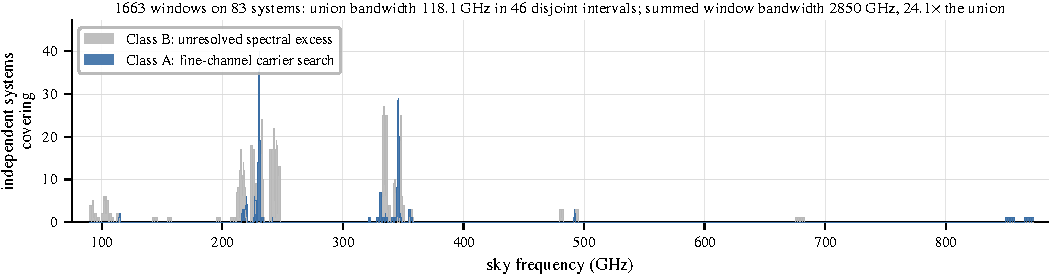
\includegraphics[width=0.99\textwidth]{figures/coverage_waterfall.pdf}
\caption{Where this survey searched: the number of independent systems
covering each sky frequency -- blue the fine-channel carrier search
(Class~A), light grey the coarse-channel spectral-excess search (Class~B).
Curves step at the searched window edges themselves, so an interval narrower
than a plotted pixel still appears. The summed window bandwidth is
$\GrossOverUnion\times$ the union.}
\label{fig:waterfall}
\end{figure*}

%% Floats that belong elsewhere: tab:blockledger is in Appendix A (its
%% headline rows are in the prose above, so the cross-reference is not a
%% pointer with no numbers beside it); tab:interesting is neither typeset nor
%% distributed -- r15-deposit, 2026-10-08: there is no deposit, so if its rows
%% are wanted by a reader they have to be printed; tab:searchspace is deleted, nothing having cited
%% it, and its counts, unions, channel widths and drift range are all
%% elsewhere in the paper.
%% Carried forward to the numbers owner: tab_interesting.tex is still
%% generated but is not in make_all.sh, and its planet column should read the
%% dated NASA Exoplanet Archive extract selfunc_v411.py uses so that one
%% definition of "confirmed planet" serves both tables.  Two display defects
%% belong in star_alias.designation: Barnard's Star prints as a SIMBAD
%% identifier with the "NAME" prefix stripped, and BD+05 1668 would read
%% better with its GJ alias beside it.
